% Copyright 2013 Nicolai Hähnle <nhaehnle@gmail.com>
%
% This work is licensed under the Creative Commons Attribution-ShareAlike 3.0
% Unported License, see http://creativecommons.org/licenses/by-sa/3.0/
%
% Among other things, this means that yes, you may take e.g. illustrations from
% the book and use them in your own work. However, (a) you must give proper
% attribution by naming me as its original author and (b) you must make your
% derivative work available under the same or similar license terms.
%
% See the Creative Commons website for the exact licensing terms.

\chapter{Arbitrary Norms and Enumeration of Lattice Points}

We have seen how to find shortest and closest vectors in a lattice
with respect to the Euclidean norm in time $2^{O(d)} \cdot \poly(b)$,
where $b$ is the encoding size of the input.
What about the related problems with respect to an arbitrary norm $\|\cdot\|$?

In the decision variant of the closest vector problem,
we are given a lattice $\Lambda \subset \R^d$,
target vector $t \in \R^d$
and target distance $r > 0$,
and we have to decide whether there is a lattice point $x \in \Lambda$
with $\|x - t\| \leq r$.
This is a lattice programming problem:
decide whether the norm ball $B_{\|\cdot\|}(t,r)$ contains a lattice point.
We have seen that such problems can be solved in
$2^{O(d \log d)} \cdot \poly(b)$ arithmetic operations
and calls to an oracle describing $B_{\|\cdot\|}(t,r)$,
where $b$ is an upper bound on the encoding size of the problem,
including the logarithm of a bound on the size of $B_{\|\cdot\|}(t,r)$.
There is a gap between this running time and
the time we could previously achieve for the Euclidean norm.

We do not know how to adapt the techniques based on Voronoi cells
since Voronoi diagrams in other norms are rather complicated.
For one thing, Voronoi cells with respect to arbitrary norms are not even convex in general.

A different approach is needed.
Suppose we could somehow enumerate the lattice points in any convex body efficiently,
by an output-sensitive algorithm,
in time $(N+1)\cdot 2^{O(d)}$
where $N$ is the number of lattice points that are found.
Then a natural algorithm for solving the shortest vector problem is as follows:
Start with a lower bound $r = r_0$ on the $\|\cdot\|$-length of a shortest vector
and enumerate lattice points in the $\|\cdot\|$-ball of radius $r$ around the origin.
If any non-zero lattice points are found, output the shortest among them.
Otherwise, multiply $r$ by a constant factor and repeat.

Due to a volume argument,
the first $\|\cdot\|$-ball to contain \emph{any} non-zero lattice points
can only contain $2^{O(d)}$ of them.
Then the overall running time is still bounded by a single-exponential factor
times the logarithm of the quality of the initial estimate $r_0$.

In this chapter,
we will visit some theory on arbitrary norms,
develop a lattice point enumeration algorithm,
and use it to solve the shortest vector problem
and approximate the closest vector problem
with respect to arbitrary norms.

This approach is based on~\cite{DPV10}
and in fact works for \emph{semi-norms} and non-symmetric convex bodies.
However, we will restrict ourselves to the case of symmetric bodies
to simplify the presentation.


\section{Norms and Convex Bodies}

The unit ball
$B_{\|\cdot\|}(0,1)$
with respect to an arbitrary norm $\|\cdot\|$
is a compact convex set of positive volume.
Furthermore, it is \emph{symmetric}
in the sense that $B_{\|\cdot\|}(0,1) = -B_{\|\cdot\|}(0,1)$.

\begin{definition}
  Let $K$ be a symmetric, compact, convex set of positive volume.
  We define the norm associated to $K$ as
  \[
    \| x \|_K := \min\{ r \geq 0 ~:~ x \in r K \}
  \]
\end{definition}


\begin{lemma}
  $\|\cdot\|_K$ is a norm.
\end{lemma}
\begin{proof}
  Since $K$ has positive volume, is symmetric and convex,
  it contains a ball $B(0,\varepsilon)$ for some $\varepsilon > 0$.
  For any $x \neq 0$, this implies $x \in \frac{\|x\|_2}{\varepsilon} K$.
  So $\|x\|_K$ is well-defined for all $x \in \R^d$
  with $\|x\|_K = 0$ if and only if $x = 0$.

  In addition, we need to show $\|\lambda x\|_K = |\lambda| \cdot \|x\|_k$
  and the triangle inequality.
  By definition and using symmetry,
  \begin{align*}
    \|\lambda x\|_K
      &= \min\{ r \geq 0 ~:~ \lambda x \in r K \}
      = \min\{ r \geq 0 ~:~ x \in \frac{r}{|\lambda|} K \}
 \\ & = \min\{ |\lambda| r \geq 0 ~:~ x \in r K \}
      = |\lambda| \cdot \|x\|_K
  \end{align*}
  Let $x, y \in \R^d$.
  We have $x \in \|x\|_K \cdot K$ and $y \in \|y\|_K \cdot K$.
  Intuitively, the idea is that
  \[
    x + y \in \|x\|_K \cdot K + \|y\|_K \cdot K = (\|x\|_K + \|y\|_K) K
  \]
  and therefore $\|x+y\|_K \leq \|x\|_K + \|y\|_K$.
  The last equality of sets holds for general convex sets.
  We only need inclusion from left to right.
  Any $z \in \lambda K + \mu K$ can be written as $z = x + y$
  with $x \in \lambda K$ and $y \in \mu K$ by definition.
  \begin{align*}
    z = x + y = \lambda \cdot \underbrace{\frac{x}{\lambda}}_{\in K}
      + \mu \cdot \underbrace{\frac{y}{\mu}}_{\in K} \in (\lambda + \mu) K
  \end{align*}
  by convexity.
\end{proof}



\section{The polar of a convex body}

\begin{definition}
  Let $K \subset \R^d$ be a convex set.
  The \emph{polar} of $K$ is defined as
  \[
    K^\star := \{ y \in \R^d ~:~ y^Tx \leq 1 \,\forall x \in K \}
  \]
\end{definition}

The polar is sometimes also called the dual of a convex body.
Even though that terminology is also useful,
for example due to the connection to dual lattices that we will see,
we prefer the term polar so as not to get confused with linear programming duality.
While the definition can be written down for arbitrary convex sets,
we will see that it is most meaningful for sets that contain $0$.

\begin{example}
  The cube $[-1,+1]^d$ is the polar of the cross polytope $\conv\{\pm e_j\}$ and vice versa.
  \begin{center}
    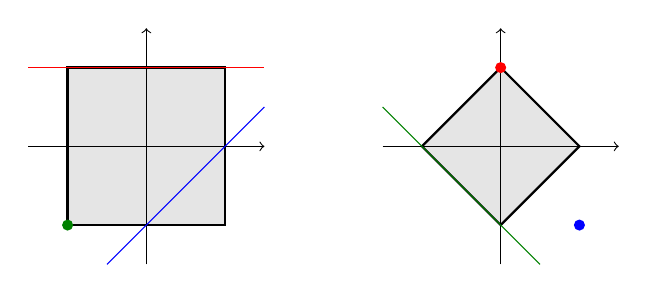
\begin{tikzpicture}
      \draw[thick,fill=black!10] (-1,-1) -- (1,-1) -- (1,1) -- (-1,1) -- cycle;
      \draw[->] (-1.5,0) -- (1.5,0);
      \draw[->] (0,-1.5) -- (0,1.5);

      \draw[thick,fill=black!10] (3.5,0) -- (4.5,-1) -- (5.5,0) -- (4.5,1) -- cycle;
      \draw[->] (3,0) -- (6,0);
      \draw[->] (4.5,-1.5) -- (4.5,1.5);

      \draw[red] (-1.5,1) -- (1.5,1);
      \fill[red] (4.5,1) circle[radius=2pt];

      \draw[blue] (-0.5,-1.5) -- (1.5,0.5);
      \fill[blue] (5.5,-1) circle[radius=2pt];

      \draw[green!50!black] (3,0.5) -- (5,-1.5);
      \fill[green!50!black] (-1,-1) circle[radius=2pt];
    \end{tikzpicture}
  \end{center}
  Valid inequalities of $K$ correspond to points in $K^\star$ and vice versa,
  as some examples in the drawing indicate.
\end{example}

\begin{lemma}
  Let $K \subseteq \R^d$ be a convex set.
  \begin{enumerate}
    \item $K^\star$ is a closed convex set that contains the origin.
    \item If $K$ is bounded, then $0 \in \operatorname{int} K^\star$.
    \item If $0 \in \operatorname{int} K$, then $K^\star$ is bounded.
    \item $K_1 \subseteq K_2$ implies $K_1^\star \supseteq K_2^\star$.
    \item $K \subseteq (K^\star)^\star$
    \item If $K$ is closed and contains the origin, then $(K^\star)^\star = K$.
  \end{enumerate}
\end{lemma}
\begin{proof}
  For the first point, observe that $K^\star$ can be written as the (infinite) intersection
  of closed half-spaces and $0 \in K^\star$ is obvious.

  For the second point, let $K \subseteq B(0, R)$
  and let $y \in B(0, 1/R)$.
  Then for all $x \in K$, one has
  \[
    y^T x \leq \|x\|_2 \|y\|_2 \leq 1
  \]
  Hence $B(0,1/R) \subseteq K^\star$.

  For the third point, suppose $B(0,\varepsilon) \subseteq K$.
  Let $y \in K^\star$.
  Observe that $x := \varepsilon \frac{y}{\|y\|_2} \in K$,
  and so we have
  \[
    1 \geq y^Tx = \varepsilon \frac{y^Ty}{\|y\|_2} = \varepsilon \|y\|_2
  \]
  This implies $\|y\|_2 \leq 1/\varepsilon$, hence $K^\star$ is bounded.

  For the fourth point, observe that $y \in K_2^\star$
  satisfies $y^Tx \leq 1$ for all $x \in K_2$.
  In particular, it satisfies $y^Tx \leq 1$ for all $x \in K_1$,
  hence $y \in K_1^\star$.

  For the fifth point,
  let $x \in K$.
  We have $y^Tx \leq 1$ for all $y \in K^\star$ (by the definition of $K^\star$)
  and so (by the definition of $(K^\star)^\star$) we have $x \in (K^\star)^\star$.

  For the last point,
  it remains to be shown that $(K^\star)^\star \subseteq K$.
  Suppose, by way of contradiction,
  that there exists a point $z \in (K^\star)^\star$ with $z \not\in K$.
  Since $K$ is closed,
  there is a hyperplane that strictly separates $z$ from $K$.
  Formally, there exists a hyperplane with equation $a^Tx = b$
  such that $a^Tx < b$ for all $x \in K$ and $a^Tz > b$.

  Since $0 \in K$, we have $b > 0$.
  By rescaling, we can ensure $b = 1$, which implies $a \in K^\star$.
  But since $a^Tz > b = 1$, this contradicts $z \in (K^\star)^\star$.
\end{proof}

\begin{lemma}
  Let $A \in \R^{d \times d}$ be an invertible matrix.
  Then $(A K)^\star = A^{-T} K^\star$.
\end{lemma}
\begin{proof}
  This follows from a simple chain of equivalences,
  the heart of which is the fact that $y^T(Ax) = (A^T y)^T x$.
\end{proof}

The polar of a convex body is related to its primal in the same way
that a dual lattice is related to its primal as per Corollary~\ref{corollary:transformed-dual-lattice}.
Indeed, when working in a lattice $\Lambda$ with respect to a norm $\|\cdot\|_K$,
we should work in its dual with respect to the norm $\|\cdot\|_{K^\star}$.
Let us extend the covering radius and the successive minima to general norms in the natural way,
where $K$ is a symmetric convex body of positive volume:
\begin{align*}
  \lambda_j(\Lambda, K) &:= \min\{ r > 0 ~:~ \dim( \Lambda \cap B_{\|\cdot\|_K}(0,r) ) \geq j \} \\
  \mu(\Lambda, K) &:= \max_{p \in \R^d} d_{\|\cdot\|_K}(p, \Lambda)
\end{align*}
We can immediately extend some of the statements from Chapter~\ref{chapter:dual-lattices}.
\begin{lemma}
  The lattice width of $K$ is related to the length of a shortest vector in the dual by
  $w(K,\Lambda) = 2\lambda_1(\Lambda^\star, K^\star)$.
\end{lemma}
\begin{proof}
  Let $y \in \Lambda^\star$.
  \begin{align*}
    w_y(K) = \max_{x \in K} y^Tx - \min_{x \in K} y^Tx = 2 \max_{x \in K} y^Tx
  \end{align*}
  by symmetry.
  Read differently, we have
  \[
    y^Tx \leq \frac{w_y(K)}{2}
  \]
  for all $x \in K$, which implies $y \in \frac{w_y(K)}{2} K^\star$.
  On the other hand, there is an $x \in K$ that satisfies the inequality with equality,
  and hence $w_y(K) / 2$ is the smallest possible factor by which $K^\star$ must be scaled to contain $y$,
  i.e. $\|y\|_{K^\star} = w_y(K) / 2$.
  Finally,
  \[
    w(K,\Lambda) = \min_{y\in K^\star\setminus 0} w_y(K) = \min_{y\in K^\star\setminus 0} 2 \|y\|_{K^\star}
      = 2 \lambda_1(\Lambda^\star, K^\star) \qedhere
  \]
\end{proof}

\begin{lemma}[Flatness Lemma]
  Suppose one has $\lambda_1^\star(\Lambda^\star, K^\star) \cdot \mu(\Lambda, K) \leq c_d$
  for all lattices $\Lambda \subset \R^d$ and symmetric convex bodies $K \subseteq \R^d$.
  Then $w(K,\Lambda) \geq 2c_d$ implies that $p + K$ contains a lattice point for every $p \in \R^d$.
\end{lemma}
\begin{proof}
  By the previous Lemma, $2c_d \leq w(K,\Lambda) = 2 \lambda_1^\star(\Lambda^\star, K^\star)$.
  This implies $\mu(\Lambda, K) \leq 1$,
  which by definition means that for every $p \in \R^d$,
  there is an $x \in \Lambda$ with $\|p - x\|_K \leq 1$.
  But then $x \in p + K$.
\end{proof}





\section{Enumerating lattice points in an ellipsoid}

Let $\Lambda \subseteq \R^d$ be a lattice and $B = B(z,r)$ a ball.
How can we quickly enumerate the points in $B \cap \Lambda$?

Recall the notion of Voronoi diagram of a lattice from Chapter~\ref{chapter:voronoi-cell}.
We can define a graph $G = (\Lambda, E)$ by saying that
\[
  xy \in E \iff x + \overline{\cV} \text{ and } y + \overline{\cV} \text{ share a facet}
\]
Equivalently, $xy \in E$ if $y - x$ is Voronoi relevant
(recall Definition~\ref{def:voronoi-relevant}).
Intuitively, this graph is the ``dual graph'' of the Voronoi diagram.
Note that the degree of each vertex is bounded by $2\cdot (2^d - 1)$
by Corollary~\ref{cor:number-of-voronoi-relevant}.
Let $G[B]$ be the graph induced by the vertices in $B \cap \Lambda$;
see Figure~\ref{fig:voronoi-graph} for an illustration.

\begin{figure}
  \begin{center}
    \begin{tikzpicture}
      \clip (-2.2,-2.3) rectangle (2.2,4.3);

      \foreach \y in {-1,0,1,2}
        \foreach \x in {-3,-2,-1,0,1,2}
          \fill ($\x*(1,0) + \y*(0.5,2)$) circle[radius=2pt];

      \foreach \y in {-2,0,2,4}
        \draw (-2.2,\y) -- (2.2,\y);
      \foreach \x in {-4,-3,...,3.01} {
        \draw ($(-1,-4) + \x*(1,0)$) -- +(2.5,10);
        \draw ($(-1.5,6) + \x*(1,0)$) -- +(2.5,-10);
      }

      \foreach \y in {-1,0,1,2}
        \foreach \x in {-4,-3,-2,-1,0,1,2}
          \draw[help lines] ($\x*(1,0) + \y*(0.5,2)$) +(0,1.0625) -- +(0.5,0.9375) -- +(0.5,-0.9375) -- +(0,-1.0625);
    \end{tikzpicture}
    \qquad
    \begin{tikzpicture}
      \clip (-2.2,-2.3) rectangle (2.2,4.3);

      \draw[fill=black!10] (-0.2,0.8) circle[radius=1.9cm];

      \foreach \y in {-1,0,1,2}
        \foreach \x in {-3,-2,-1,0,1,2}
          \fill[help lines] ($\x*(1,0) + \y*(0.5,2)$) circle[radius=2pt];

%       \foreach \y in {-2,0,2,4}
%         \draw[help lines] (-2.2,\y) -- (2.2,\y);
%       \foreach \x in {-4,-3,...,3.01} {
%         \draw[help lines] ($(-1,-4) + \x*(1,0)$) -- +(2.5,10);
%         \draw[help lines] ($(-1.5,6) + \x*(1,0)$) -- +(2.5,-10);
%       }

      \foreach \y in {-1,0,1,2}
        \foreach \x in {-4,-3,-2,-1,0,1,2}
          \draw[help lines] ($\x*(1,0) + \y*(0.5,2)$) +(0,1.0625) -- +(0.5,0.9375) -- +(0.5,-0.9375) -- +(0,-1.0625);

      \foreach \p in {(0,0),(-1,0),(1,0),(-1.5,2),(-0.5,2),(0.5,2)}
        \fill \p circle[radius=2pt];
      \draw (-1.5,2) -- (-1,0) -- (1,0) -- (0.5,2) -- cycle;
      \draw (-1,0) -- (-0.5,2) -- (0,0) -- (0.5,2);
    \end{tikzpicture}
  \end{center}
  \caption{The dual graph of the Voronoi diagram of a lattice and the subgraph induced by a disk.}
  \label{fig:voronoi-graph}
\end{figure}

\begin{lemma}
  $G[B]$ is connected.
\end{lemma}
\begin{proof}
  Let $B = B(z,r)$ and let us briefly argue that we may assume,
  by a simple perturbation argument,
  that $z$ has a unique closest vector $x^\star \in \Lambda$.
  First, we can choose $\varepsilon > 0$ such that there is no lattice point at distance
  less than $\varepsilon$ outside $B$.
  Then, if $z$ has multiple closest vectors, we may choose one of them as $x^\star$
  and move $z$ by $\varepsilon/2$ towards it to obtain a new center $z'$.
  The ball $B(z', r + \varepsilon/2)$ contains the same lattice points as $B$,
  and $z'$ has a unique closest vector, see Figure~\ref{fig:perturbation-center-of-ball-keeps-lattice-points}.

  \begin{figure}
    \begin{center}
      \begin{tikzpicture}
        \clip (-2.2,-2.3) rectangle (2.2,4.3);

        \coordinate (z) at (-0.5,0.9375);
        \coordinate (z') at (-0.45,0.84375);

        \draw[fill=black,fill opacity=0.1] (z) circle[radius=1.3cm];
        \draw[fill=black,fill opacity=0.1] (z') circle[radius=1.4cm];

        \foreach \y in {-1,0,1,2}
          \foreach \x in {-3,-2,-1,0,1,2}
            \fill ($\x*(1,0) + \y*(0.5,2)$) circle[radius=2pt];

        \foreach \y in {-1,0,1,2}
          \foreach \x in {-4,-3,-2,-1,0,1,2}
            \draw[help lines] ($\x*(1,0) + \y*(0.5,2)$) +(0,1.0625) -- +(0.5,0.9375) -- +(0.5,-0.9375) -- +(0,-1.0625);

        \fill (z) circle[radius=2pt] node[above left] {$z$};
        \draw (z) -- +(20:1.3cm);
        \fill (z') circle[radius=2pt] node[below left] {$z'$};
        \draw (z') -- +(20:1.4cm);
      \end{tikzpicture}
    \end{center}
    \caption{Perturbing $z$ results in a ball containing the same lattice point whose center has a unique closest vector.}
    \label{fig:perturbation-center-of-ball-keeps-lattice-points}
  \end{figure}

  We will show that every $x \in \Lambda \cap B$ is connected to $x^\star$ by a path in $G[B]$.
  Choose a maximal sequence $x = x_0, x_1, \ldots, x_N \in \Lambda$ satisfying
  \begin{enumerate}
    \item $x_{j+1} - x_j$ is Voronoi relevant and
    \item $\|x_{j+1} - z\|_2 < \|x_j - z\|_2$.
  \end{enumerate}
  That is, greedily walk from $x$ along edges to get closer to $z$.
  By maximality of the sequence (equivalently: by the fact that we cannot continue greedily from $x_N$), we have
  \[
    \|x_N - z\|_2 \leq \|x_N - (z + v)\|_2
  \]
  for all Voronoi relevant vectors $v$.
  This means $x_N \in z + \overline{\cV}$,
  which implies $x_N = x^\star$ since $z$ has a unique closest vector.
  That is, we found a path from $x$ to $x^\star$ in $G[B]$.
\end{proof}

This suggests a straightforward approach to enumerating the lattice points in a ball.
First, find a closest vector to the center of the ball.
Then apply breadth-first search in $G[B]$.

There is a subtle difficulty of implementation.
Breadth-first search is well-known to take linear time when a graph is given explicitly.
However, in our case, $G[B]$ is only known implicitly.
When visiting a vertex $x \in B \cap \Lambda$,
we can easily enumerate the \emph{coordinates} of its neighbours since we know the Voronoi relevant vectors.
However, it is not so obvious how to check whether that neighbour has already been visited or not.

A simple work-around is to store all visited vertices in an efficient data structure
such as a balanced binary search tree.
Alternatively, one might visit vertices in the order of increasing distance from $x^\star$ (or $z$).
Both methods work,
although both require $O(\log |B \cap \Lambda|)$-time operations for associated checks
such as lookups in binary search trees or maintenance of a heap.

\begin{lemma}
  $\log |B \cap \Lambda| \leq \poly(b)$,
  where $b$ is the encoding size of $B$ and $\Lambda$.
\end{lemma}
\begin{proof}
  Let $B = B(z,r)$.
  Recall that we assume rational lattices for computational purposes.
  By multiplying with least common denominators, we can assume $\Lambda \subset \Z^d$ for simplicity.
  Then $\lambda_1 \geq 1$, and hence the balls of radius $1/2$ around lattice points are disjoint.
  We obtain
  \[
    |B \cap \Lambda| \cdot \vol B(0,\frac{1}{2}) \leq \vol B(z,r) = 2^d r^d \vol B(0,\frac{1}{2})
  \]
  This implies the result.
\end{proof}

That is, we can fold the running time that is required to maintain the assorted data structures
into the catch-all factor of $\poly(b)$ that the running times of all our algorithms have anyway,
and obtain:

\begin{theorem}
  There is an algorithm that,
  given a lattice $\Lambda \subset \R^d$ and an ellipsoid $E$,
  enumerates all points in $E \cap \Lambda$ in time
  $(1 + |E \cap \Lambda|) 2^{O(d)} \poly(b)$.
\end{theorem}
\begin{proof}
  We can assume that $E$ is a ball by applying a linear transformation to both $E$ and $\Lambda$.
  The rest follows from the discussion above.
\end{proof}





\section{Enumeration by ellipsoid coverings}

Given that we know how to enumerate lattice points in ellipsoids,
our overall strategy for enumerating lattice points in arbitrary convex bodies $K$
will be to cover $K$ by ellipsoids.

\begin{figure}
  \begin{center}
    \begin{tikzpicture}
      \foreach \y in {0,1}
        \foreach \x in {0,1,...,36.01} {
          \fill ($\y*(1,-2.4) + \x*(0.1,0.02)$) circle[radius=.5pt];
        }
      
      \draw[thick,fill=black!10] (0.5,0.05) -- (2.5,0.45) -- node[right] {$K$} (1.5,-0.35) --cycle;
    \end{tikzpicture}
  \end{center}
  \caption{There may be arbitrarily many lattice points in a neighborhood of $K$.}
  \label{fig:sparse-dense-close-to-K}
\end{figure}

Such a cover will usually not be exact, that is,
the covering ellipsoids may contain lattice points that are not in $K$.
In fact, there may be arbitrarily many lattice points just outside of $K$
even when $K$ does not contain any lattice point,
see Figure~\ref{fig:sparse-dense-close-to-K}.
We cannot hope to achieve a running time proportional to $|K \cap \Lambda|$ in this case.

\begin{definition}
  Let $K \subseteq \R^d $ be a bounded convex body and let $\Lambda \subset \R^d$ be a lattice.
  We define $G(K,\Lambda) := \max_{p \in \R^d} |(p + K) \cap \Lambda|$.
\end{definition}

Our goal will be to enumeration points in $K$ in time proportional to $G(K, \Lambda)$.

\begin{example}
  Let us see why we cannot just enumerate points in (an approximation of)
  a smallest enclosing ellipsoid.
  Consider the cross-polytope $P = \conv\{\pm e_j\}$,
  whose smallest enclosing ellipsoid is the unit ball.
  \begin{center}
    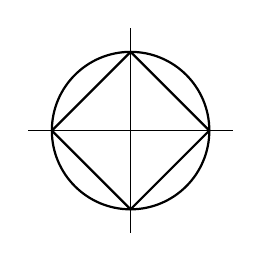
\begin{tikzpicture}
      \draw (-1.3,0) -- (1.3,0);
      \draw (0,-1.3) -- (0,1.3);
      \draw[thick] (-1,0) -- (0,1) -- (1,0) -- (0,-1) -- cycle;
      \draw[thick] (0,0) circle[radius=1cm];
    \end{tikzpicture}
  \end{center}
  The cross-polytope is a union of $2^d$ unit simplices,
  one for each orthant.
  Hence we can compute its volume as
  \[
    \vol(P) = 2^d \cdot \frac{1}{d!} \sim 2^d \frac{1}{\sqrt{2\pi d}} \left( \frac{e}{d} \right)^d
  \]
  where we use Stirling's approximation for the factorial.
  The volume of the Euclidean unit ball is
  \[
    \frac{\pi^{d/2}}{\Gamma(d/2 + 1)} \sim \pi^{d/2} \frac{1}{\sqrt{\pi d}} \left( \frac{2e}{d} \right)^{d/2}
  \]
  For sufficiently dense lattices, we have
  $|K \cap \Lambda| \sim \frac{\vol(K)}{\det(\Lambda)}$ (see the exercises).
  So let us compare volumes:
  \[
    \frac{\vol(B)}{\vol(P)} \sim \frac{\pi^{d/2} \sqrt{2}}{2^{d/2}} \left( \frac{d}{e} \right)^{d/2} = 2^{\Omega(d \log d)}
  \]
  For a sufficiently dense lattice $\Lambda$,
  the same relation holds for $|B \cap \Lambda|$ and $|P \cap \Lambda|$.
  That is, enumerating the points in $B$ necessarily introduces a $2^{\Omega(d \log d)}$ factor into the running time,
  which is too wasteful for our purposes.
\end{example}

\begin{example}
  \label{example:cover-the-ball-with-cubes}
  Let us now consider that case where $P = [-1,+1]^d$ is a cube.
  The smallest volume enclosing ellipsoid is the ball $B = B(0, \sqrt{d})$.
  \begin{center}
    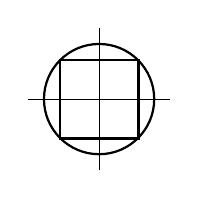
\begin{tikzpicture}
      \draw (-.9,0) -- (.9,0);
      \draw (0,-.9) -- (0,.9);
      \draw[thick] (-.5,-.5) -- (-.5,.5) -- (.5,.5) -- (.5,-.5) -- cycle;
      \draw[thick] (0,0) circle[radius=.7cm];
    \end{tikzpicture}
  \end{center}
  Comparing their volumes, we obtain $\vol(P) = 2^d$ and
  \[
    \vol(B) = \sqrt{d}^d \frac{\pi^{d/2}}{\Gamma(d/2+1)} \sim \frac{d^{d/2} \pi^{d/2}}{\sqrt{\pi d}} \left( \frac{2e}{d} \right)^{d/2}
      = \frac{(2 e \pi)^{d/2}}{\sqrt{\pi d}}
  \]
  The ratio between these volumes is $2^{O(d)}$.

  How many more lattice points are contained in $B$ than in $P$?
  We can bound this number by observing that $B$ can be covered by translated copies of $P$,
  see Figure~\ref{fig:cover-B-by-P}.
  Let
  \[
    S := \{ x \in 2\Z^d ~:~ (x + P) \cap B \neq \emptyset \}
  \]
  We have
  \[
    |B \cap \Lambda| \leq |S| \cdot G(P, \Lambda).
  \]
  because $B \subseteq S + P$.
  Furthermore,
  since the length of the diagonal of $P$ is $2\sqrt{d}$
  we have $x + P \subseteq B + B(0,2\sqrt{d}) = B(0,3\sqrt{d})$ for every $x \in S$.
  Using the disjointness of the $x + P$ (up to sets of measure $0$),
  we compute
  \[
    |S| \cdot 2^d = |S| \cdot \vol P \leq \vol B(0,3\sqrt{d}) \sim 3^d d^{d/2} \cdot \frac{\pi^{d/2}}{\sqrt{\pi d}} \left( \frac{2e}{d} \right)^{d/2}
    = 2^{O(d)}
  \]
  and hence $|S| = 2^{O(d)}$ and $|B \cap \Lambda| \leq 2^{O(d)} \cdot G(P, \Lambda)$.
  
  This means that we may enumerate the lattice points in a cube
  (and, by linear transformation, in a parallelepiped)
  by enumerating the lattice points in the smallest enclosing ellipsoid.
\end{example}
\begin{figure}
  \begin{center}
  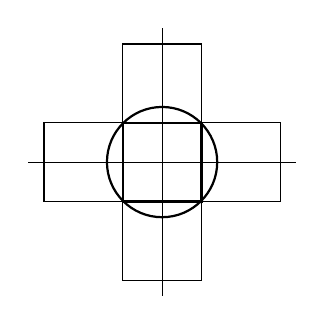
\begin{tikzpicture}
    \draw (-1.7,0) -- (1.7,0);
    \draw (0,-1.7) -- (0,1.7);
    \draw[thick] (-.5,-.5) -- (-.5,.5) -- (.5,.5) -- (.5,-.5) -- cycle;
    \foreach \x / \y in {1/0,-1/0,0/1,0/-1}
      \draw (\x,\y) +(-.5,-.5) -- +(-.5,.5) -- +(.5,.5) -- +(.5,-.5) -- cycle;
    \draw[thick] (0,0) circle[radius=.7cm];
  \end{tikzpicture}
  \end{center}
  \caption{Bounding the number of lattice points in $B$ in terms of $G(P,\Lambda)$.}
  \label{fig:cover-B-by-P}
\end{figure}

\begin{definition}
  Let $A, B \subset \R^d$ be convex bodies.
  We define
  \[
    N(A,B) := \min\{ |S| ~:~ A \subseteq S + B \}
  \]
\end{definition}

\begin{example}
  We saw previously that for $P = [-1,+1]^d$ and $B$ a ball of radius $\sqrt{d}$,
  one has $N(P,B) = 1$ and $N(B,P) = 2^{O(d)}$.
\end{example}

For the remainder of this section, we will work towards a proof of the following:
\begin{theorem}
  \label{thm:enumerate-in-K-given-E}
  There is an algorithm that, given a lattice $\Lambda \subset \R^d$,
  a convex body $K \subset \R^d$, and an ellipsoid $E \subset \R^d$,
  enumerates all points of $K \cap \Lambda$ (possibly multiply)
  in time $N(K,E) \cdot N(E,K) \cdot G(K,\Lambda) \cdot 2^{O(d)} \cdot \poly(b)$.
\end{theorem}

\begin{lemma}
  Given a convex body $K \subset \R^d$ and an ellipsoid $E \subset \R^d$,
  one can compute a set $S \subset \R^d$ satisfying
  (i) $K \subseteq S + E$ and (ii) $|S| \leq 2^{O(d)} N(K,E)$
  in time $N(K,E) \cdot 2^{O(d)} \cdot \poly(b)$.
\end{lemma}
\begin{proof}
  By a linear transformation,
  we may assume $E = B(0,\sqrt{d})$.
  We generalize the tiling approach of Example~\ref{example:cover-the-ball-with-cubes}.
  Let $C := [-1,+1]^d$ and
  \[
    S := \{ x \in 2\Z^d ~:~ (x + C) \cap \operatorname{int} K \neq \emptyset \}
  \]
  First, one easily sees that $K \subseteq S + E$.
  
  To show the desired bound on $|S|$,
  let $S^\star$ be a set of $N(K,E)$ points
  such that $K \subseteq S^\star + E$.
  By forming a Minkowski sum on both sides of the set inclusion, we get
  \[
    K + B(0,2\sqrt{d}) \subseteq S^\star + \underbrace{E + B(0,2\sqrt{d})}_{= B(0,3\sqrt{d})}
  \]
  On the other hand,
  \[
    S + C \subseteq K + B(0,2\sqrt{d})
  \]
  since the length of the diagonal of $C$ is $2\sqrt{d}$.
  Using the fact that the translates of $C$ are disjoint (up to sets of measure $0$),
  we get
  \[
    \vol(K + B(0,2\sqrt{d})) \geq |S| \cdot \vol C = |S| \cdot 2^d
  \]
  On the other hand,
  \[
    \vol(K + B(0,2\sqrt{d})) \leq |S^\star| \cdot \vol B(0,3\sqrt{d})
    = N(K,E) \cdot 3^d d^{d/2} \cdot \frac{\pi^{d/2}}{\Gamma(d/2 + 1)}
  \]
  Putting these two inequalities together and using Stirling's approximation
  yields $|S| \leq N(K,E) \cdot 2^{O(d)}$.
  
  Computing the set $S$ is fairly straightforward.
  We can round any point $x \in \operatorname{int} K$ to the closest vector in $2 \Z^d$
  to obtain an initial point $x^\star \in S$.

  We claim that the dual graph on $S$,
  that is,
  the graph $G = (S,E)$ with $xy \in E$ if and only if $x+C$ and $y+C$,
  is connected.

  We show the claim by an argument similar to the algorithm~\proc{CVP-via-Voronoi-Simple}
  of section~\ref{sec:svp-cvp-via-voronoi}.
  Let $x \neq y \in S$.
  Let $x' \in (x+C) \cap \operatorname{int} K$ and $y' \in (x+C) \cap \operatorname{int} K$.
  If necessary, we can perturb $x'$ and $y'$ slightly
  so that the line segment $x'y'$
  does not intersect a lower-dimensional face of any of the cubes $z + C$ for $z \in S$.
  The line segment $x'y'$ stays within $\operatorname{int} K$ due to convexity,
  and so it naturally induces a path that connects $x$ and $y$ in $G$.

  This means that we can perform a breadth-first search starting at $x^\star$ to find all vertices of the graph.
  At each vertex of $G$, there are $2d$ potential neighbours for which we have to check
  whether they have already been seen and whether they are in the graph.
  The latter is a simple linear programming problem.
  Overall, we can compute $S$ in the desired running time.
\end{proof}

\begin{proof}[Theorem~\ref{thm:enumerate-in-K-given-E}]
  First, use the algorithm of the Lemma
  to construct a covering of $K$ by $N(K,E) \cdot 2^{O(d)}$ translates of $E$ using the algorithm of the Lemma.
  Recall that each translate of $E$ can be covered by $N(E,K)$ translates of $K$,
  and so each translate contains at most $N(E,K) \cdot G(K,\Lambda)$ lattice points.
  We can enumerate these points for every translate using the algorithm of the previous section.
  
  The overall running time is dominated by the enumeration,
  which is precisely as desired.
\end{proof}


\section{M-ellipsoids}



\section*{Exercises}

\begin{enumerate}
  \item Show: $K^\star = K$ if and only if $K$ is the closed Euclidean unit ball.
  
  \item Let $K \subset \R^d$ be a convex body of positive volume.
    The goal of this exercise is to show
    that the number of lattice points in $K$ is asymptotically equal to $\vol(K) / \det(\Lambda)$
    for dense lattices.
  \begin{enumerate}[(a)]
    \item Let $\varepsilon > 0$ and consider the tiling of $\R^d$
      obtained by placing the cube $C_\varepsilon := [-\varepsilon/2, +\varepsilon/2]^d$ at
      the points $\varepsilon \Z^d$.
      Furthermore, let
      \begin{align*}
        L_\varepsilon &:= \{x \in \varepsilon \Z^d ~:~ x + C_\varepsilon \subseteq K \} \\
        U_\varepsilon &:= \{x \in \varepsilon \Z^d ~:~ (x + C_\varepsilon) \cap K \neq \emptyset \}
      \end{align*}
      Show: $|L_\varepsilon| \leq |K \cap \varepsilon \Z^d| \leq |U_\varepsilon|$ and
        $|L_\varepsilon| \leq \frac{\vol(K)}{\varepsilon^d} \leq |U_\varepsilon|$.
    
    \item Which of the inequalities in part (a) are tight?

    \item Show: There is a constant $c_K > 0$ that depends on $K$
      such that for all sufficiently small $\varepsilon > 0$ one has $|L_\varepsilon| \geq c_K \frac{\vol(K)}{\varepsilon^d}$.
      
      \emph{Hint:} Scale $K$ around an interior point.
    
    \item Show: $\lim_{\varepsilon \to 0} \frac{|U_\varepsilon|}{|L_\varepsilon|} = 1$.
    
    \emph{Hint:} You may use the fact that
      $\lim_{\varepsilon \to 0} \frac{\vol(\partial K + B(0,\varepsilon))}{2\varepsilon} = \vol_{d-1}(\partial K)$.

    \item Let $\Lambda \subset \R^d$ be a lattice.
      Show: $\lim_{\varepsilon \to 0} \frac{\vol(K)}{\varepsilon^d \det\Lambda |K \cap \varepsilon \Lambda|} = 1$.
  \end{enumerate}
\end{enumerate}
